\sectionframe{Minimal Reproducing Model}

\section{Minimal Reproducing Model}

\begin{frame}{Minimal Reproducing Model Parameter Effects}
    \begin{figure}
        \centering
        \subfloat[Effect of $p_x$]{\includegraphics[height=0.6\textheight]{60_MinimalRepr/ParameterEffects/p_x/illustration.png}}
        \subfloat[Effect of $p_y$]{\includegraphics[height=0.6\textheight]{60_MinimalRepr/ParameterEffects/p_y/illustration.png}}
        \caption{Effects of the Individual Parameters on the Function of the Minimal Reproducing Model}
    \end{figure}
\end{frame}
